%%%%%% Preamble %%%%%%
\documentclass[sigconf, anonymous, 9pt, nonacm]{acmart}
%anonymous
% \AtBeginDocument{%
%   \providecommand\BibTeX{{%
%     \normalfont B\kern-0.5em{\scshape i\kern-0.25em b}\kern-0.8em\TeX}}}


% --- tighten vertical space above every displayed equation by 0.3ex ---
\makeatletter
% 备份原始长度,万一日后想恢复
\newlength\orig@abovedisplayskip
\newlength\orig@abovedisplayshortskip

\AtBeginDocument{%
  % 保存原值
  \setlength{\orig@abovedisplayskip}{\abovedisplayskip}%
  \setlength{\orig@abovedisplayshortskip}{\abovedisplayshortskip}%
  % 统一减 0.3ex
  \setlength{\abovedisplayskip}
            {\dimexpr\orig@abovedisplayskip-0.45ex\relax}%
  \setlength{\abovedisplayshortskip}
            {\dimexpr\orig@abovedisplayshortskip-0.45ex\relax}%
}
\makeatother



% \def\baselinestretch{0.98}

%%%%%% End Copyright Block %%%%%%
\usepackage{url}
\urlstyle{sf}
\usepackage{xcolor}
\usepackage{color}
\usepackage{graphics}
\usepackage{graphicx}
\usepackage{multirow}
\usepackage{xspace}
\usepackage{enumitem}
\usepackage{subcaption}
\usepackage{balance}
\usepackage{acmart-taps}
\usepackage{booktabs}
\usepackage{marvosym}
\usepackage{amsmath}
\usepackage{algorithm}
\usepackage{algorithmic}
\usepackage{caption}
\usepackage{booktabs}
\usepackage{multirow}\usepackage[most]{tcolorbox}
\usepackage[subtle]{savetrees}
% \def\baselinestretch{0.98}

\newcommand{\sys}{AD-Moments\xspace}
%%%%%% End Preamble %%%%%%
\begin{document}

% \title[AD-Moments: Leveraging LLM to Grasp Personalized Behavioral Anomaly Highlights for Alzheimer's Monitoring]
% {
% AD-Moments: Leveraging LLM to Grasp Personalized Behavioral Anomaly Highlights for Alzheimer's Monitoring}
%\title{\sys: Grasping Personalized Temporal Digital Biomarkers of Alzheimer's Patients via Edge-LLM Collaboration}
\title{\sys: Leveraging LLM to Grasp Personalized Behavioral Anomaly Highlights for Alzheimer's Monitoring}
% Context-Aware
%%%%%% Regular Author Block %%%%%%
\author{Heming Fu$^{1, 2}$, Hongkai Chen$^2$, Shan Lin$^1$~\textsuperscript{\Letter}, Guoliang Xing$^2$~\textsuperscript{\Letter}}
\affiliation{%
 \institution{$^1$Stony Brook University, $^2$The Chinese University of Hong Kong}
 \country{\{heming.fu, shan.x.lin\}@stonybrook.edu, \{hkchen, glxing\}@ie.cuhk.edu.hk}
}
%\authornote{\textsuperscript{\Letter}Co-Corresponding Authors.}
%\def\thefootnote{$^\dagger$}\footnotetext{Co-corresponding authors}\def\thefootnote{\arabic{footnote}}

% \renewcommand{\shortauthors}{Anonymous et al.}
\renewcommand{\shortauthors}{H. Fu et al.}

%%%%%% End Regular Author Block %%%%%%
%%%%%% End Short Author Block %%%%%%

% Add color command for revisions
\newcommand{\revised}[1]{\textcolor{blue}{#1}} % main revision
\newcommand{\data}[1]{\textcolor{red}{#1}} % need to be updated

\begin{abstract}


Alzheimer's disease (AD) is a growing global health challenge, necessitating elderly behavioral monitoring for early detection. Existing approaches typically aggregate behavioral statistics, such as average sleep onset time and daily walking duration, resulting in the loss of crucial temporal behavioral patterns, such as repeatedly checking the same location, and missing anomalous episodes where early AD symptoms manifest. 
To address this limitation, we develop \sys, 
the first system designed to grasp personalized temporal digital biomarkers indicative of AD using LLM. 
First, we develop temporal models that identify coarse-grained behavioral segments defined within a four-dimensional space (CTMS: Circadian-Task-Movement-Social), where patients' behaviors from the videos deviate from normal baselines. 
Next, the identified segments are analyzed by a medical literature-augmented large language model (LLM) to precisely refine anomaly boundaries for extracting AD manifestation episodes, i.e., temporal digital biomarkers. 
Last, the LLM uses retrieval-augmented generation (RAG) with a dedicated medical knowledge base to reason about clinically relevant interpretations of the temporal digital biomarkers, which, combined with individual variability, guides the parameterization of temporal models, enabling continuous, closed-loop personalization.
%We implemented and deployed \sys in the homes of 99 elders, collecting four weeks of continuous activity data per participant. Evaluation shows that cognitively impaired individuals exhibited 3.69× more AD manifestation episodes than normal elders, which enables the identification of early AD with 88.9\% sensitivity and an AUC of 0.94, outperforming traditional statistical baselines.
\revised{We collected continuous activity data from 99 elders over four weeks per participant and conducted offline evaluation.} Results show that cognitively impaired individuals exhibited 1.61× more AD manifestation episodes than normal elders, which enables the identification of early AD with 84.6\% sensitivity, outperforming traditional statistical baselines. The sample activity sequences of elders and our implementation are available at \href{https://github.com/HermesRY/AD-Moments}{\texttt{https://github.com/HermesRY/AD-Moments}}.


\end{abstract}



\maketitle






\section{Introduction}
\label{sec:intro}

\begin{figure}[t]
\centering
\includegraphics[width=0.85\columnwidth]{figures/example.jpg}
\caption{While statistical-based approaches count activities for AD progression signs, \sys detects anomalous behavioral patterns for temporal digital biomarkers indicating cognitive impairment.}
\label{fig:example}
\vspace{-2.1em}
\end{figure}

Alzheimer's disease (AD) affects over 50 million people worldwide with an economic burden exceeding \$1 trillion annually~\cite{WHO2024,ADI2024}. Early detection is crucial as cognitive decline becomes increasingly irreversible in later stages~\cite{Rasmussen2019EarlyDiagnosis,Porsteinsson2021Diagnosis}. Current clinical diagnostics rely on periodic cognitive assessments (e.g., MMSE~\cite{Folstein1975_MMSE}, CDR~\cite{Hughes1982_CDR}) or expensive neuroimaging (MRI, PET scans).
% , which miss gradual behavioral changes between visits and remain inaccessible for continuous monitoring~\cite{Folstein1975_MMSE,Hughes1982_CDR,wexler2023medicare}. 
These intermittent evaluations may fail to capture daily behavioral patterns where early cognitive symptoms first manifest.
Recent ambient sensing systems enable continuous behavioral monitoring for AD detection~\cite{Boyle2025Activity}, however, they have several major limitations. First, 
% current systems like ADMarker
statistics-based systems~\cite{ouyang2024ADMarker} lose  information of temporal patterns in patients' behaviors by aggregating behaviors into statistical features.
For example, they count total walking duration or average sleep time but might miss the sequential patterns revealing cognitive dysfunction~\cite{Grammatikopoulou2024SmartHomeAD}. Consider an elderly person who walks to a cabinet, pauses in confusion, and returns empty-handed (see example in Figure~\ref{fig:example}). 
Statistics-based approaches might consider this normal walking activity because the total walking time seems healthy. 
However, such anomalous behavioral patterns can be high-risk indicators for early AD, as executive dysfunction manifests more frequently in disrupted activity flow rather than activity counts~\cite{Rasmussen2019EarlyDiagnosis,kirova2015working,guarino2019executive}. 
% Second, a critical gap exists between sensing outputs and clinical interpretation for AD diagnosis. 
Second, most existing systems~\cite{Civitarese2025SERENADE} lack medical interpretation of sensing outputs, which might may cause edge models to either misidentify essential behavioral segments or recognize unnecessary ones.
% for AD diagnosis 
For instance, they may provide behavioral metrics like ``nighttime activity increased 23\% in monitoring dashboard'' but cannot distinguish whether this represents pathological wandering requiring attention or harmless insomnia that should be ignored~\cite{kamil2021detection}. 
Third, individual variability can significantly affect whether specific behaviors should be considered anomalous or normal, causing models trained on average behavioral patterns to fail to capture person-specific cognitive decline. 
For example, a night owl's normal 2am activity gets flagged as pathological wandering, while an early bird's genuine 4am confusion episodes are dismissed as normal behavior~\cite{populationdigitalhealth, peterson2017personalized}. 

% 1. cannot rely on statistics
% solution: find temporal DB from segments using LLM
% 2. do not know what the sensed pattern means, which can lead to recognize unnecessary or mis-recognize necessary behavior segments in edge models
% solution: use medical interpretation from LLM to guide/update edge models
% 3. individual variability can significantly affect the pathology of some behaviors (anomalous or not)
% solution: use individual variability to guide/update edge models

To address these challenges, we develop \sys, the first system that identifies personalized temporal digital biomarkers indicative of early AD in videos of daily living.
Our key insight is that \emph{human manifests signs of cognitive decline in not only activity statistics but also temporal behavior patterns.}
First, we develop task-specific models with temporal encoders that analyze the sequential relationships between activities. 
We propose a novel four-dimensional behavioral space (CTMS: Circadian-Task-Movement-Social) with multi-scale analysis that captures micro-level transitions (a pattern of \emph{``walk$\rightarrow$pause$\rightarrow$walk''} indicates forgotten intent), meso-level patterns (repeated unsuccessful task attempts), and macro-level disruptions (irregular circadian activity patterns) to identify coarse-grained behavioral segments that deviate from normal baselines.
% address the temporal information loss. 
% NExt, the identified segments are analyzed by a medical literature-augmented large language model (LLM) to precisely refine anomaly boundaries for extracting AD manifestation episodes, i.e., temporal digital biomarkers???????
% Last, the LLM uses retrieval-augmented generation (RAG) with a dedicated medical knowledge base to reason about clinically relevant interpretations of the temporal digital biomarkers, which, combined with individual variability, guides the parameterization of edge models, enabling continuous, closed-loop personalization. (need updated) 
Next, we integrate medical knowledge through LLM augmentation to analyze these segments and refine the anomaly boundaries. 
When the temporal intervals of cognitive symptoms are detected, the LLM extracts fine-grained video segments as AD manifestation episodes, which serves as temporal digital biomarkers for subsequent early detection.
Last, the LLM generates clinical interpretations through medical reasoning by retrieving relevant medical literature to contextualize observed behavioral patterns.
Based on accumulated evidence of individual-specific AD manifestation patterns, the LLM dynamically adjusts CTMS encoder attention weights. 
This bi-directional framework enables continuous adaptation to individual cognitive decline patterns, achieving personalized monitoring.
\revised{We collected continuous activity data from 99 elders over a four-week period per participant. Offline evaluation demonstrates that cognitively impaired individuals exhibit significantly more frequent AD manifestation episodes compared to cognitively normal elderly.}
Our system achieved 0.688 F1-Score and 84.6\% sensitivity of identifying early AD. Strong correlations with clinical assessments (e.g., MoCA~\cite{Nasreddine2005MoCA}) validate the clinical relevance of our temporal digital biomarkers.

Our main contributions are:
\begin{itemize}
\item We develop \sys, the first system that identifies temporal digital biomarkers of patients with Alzheimer's disease in activities of daily living.
% from CTMS behavioral space for Alzheimer's monitoring. 
\item We propose a four-dimensional behavioral space (CTMS: Circadian-Task-Movement-Social) to define coarse-grained segments that deviate from normal baselines. These segments are further refined at anomaly boundaries by an LLM to extract AD manifestation episodes, serving as temporal digital biomarkers for early AD detection.

% \item We leverage LLM augmented with medical literature to guide edge model multi-head attention weights for personalization, ensuring adaptation to individual variability while providing medical reasoning for AD clinical interpretation.
\item We design a continuous, closed-loop personalization mechanism for CTMS temporal encoders, using clinical interpretations from our medical LLM.
This parameterization also accounts for individual variability in early AD detection.

% the LLM uses retrieval-augmented generation (RAG) with a dedicated medical knowledge base to reason about clinically relevant interpretations of the temporal digital biomarkers, which, combined with individual variability, guides the parameterization of edge models, enabling continuous, closed-loop personalization.

%\item We implemented and tested our system on 99 elderly participants over four weeks, demonstrating strong performance in recognizing AD manifestation episodes and identifying early AD with robust clinical correlations, outperforming traditional baselines.
\item \revised{We conducted data collection from 99 elders' homes over four weeks and performed offline evaluation}, demonstrating strong performance in recognizing AD manifestation episodes and identifying early AD with robust clinical correlations, outperforming traditional baselines.
\end{itemize}



\section{System Design}
\label{sec:design}

In this section, we describe the system design of \sys.

\subsection{System Overview}

\begin{figure}[t]
\centering
\includegraphics[width=1\columnwidth]{figures/ADmoments.pdf}
\caption{Overview of \sys. 
From the daily activities of elders, CTMS temporal model detect anomalous behavior segments that deviate from normal baselines.
A literature-augmented LLM use the detected behavior segments to extract AD manifestation episodes, i.e., temporal digital biomarkers, and provide clinical interpretations.
Combined with individual variability, these clinical interpretations guide the parameterization of
CTMS temporal encoders, enabling continuous, closed-loop personalization. }
\label{fig:system_overview}
\vspace{-1em}
\end{figure}
% \vspace{-1em}

%\sys monitors 22 activities of daily living (ADL) through a depth cameras, as detailed in Table~\ref{tab:activities}. 
\sys analyzes 22 activities of daily living (ADL) of elders, as detailed in Table~\ref{tab:activities}.
These activities span basic ADL (BADL) such as walking and eating, instrumental ADL (IADL) including cleaning and grooming, and social interactions (SI) like phone calls. 
As shown in Fig.~\ref{fig:system_overview}, \sys analyzes activity sequence through CTMS temporal encoders to recognize anomalous behavior segments that deviate from normal baselines. 
The activities are processed at three temporal scales: micro-level for immediate cognitive lapses, meso-level sequences for task execution patterns, and macro-level for circadian disruptions.
Then, a medical literature-augmented LLM helps extract precise AD manifestation moments from the detected behavior segments to identify temporal digital biomarkers, outputting refined timestamps and clinical interpretations via retrieval-augmented generation (RAG).
Lastly, these interpretations, combined with accumulated individual variability patterns, dynamically adjust CTMS temporal encoder attention weights (e.g., $\alpha_{c}$: 0.25$\rightarrow$0.40) for personalization in a continuous, closed-loop fashion.
% 参考abstract,同时要提输入,输出,硬件
%1. use edge find segment
%2. find temporal db
%3. use interpretation and varibility to update edge. form a contin, closed-loop personalzation.

% Each activity category manifests decline at different disease stages and contributes to specific behavioral dimensions. 


% The bi-directional design enables collaborative intelligence: edge models cast a wide net to detect potential anomalies efficiently, while LLM refines these detections to extract precise AD manifestation episodes and guides personalization by adjusting dimension attention weights based on accumulated behavioral evidence. This creates an adaptive system that focuses on person-specific decline patterns while maintaining consistent evaluation criteria.

\begin{table}[t]
\centering
\scriptsize
\begin{tabular}{@{}p{3.8cm}p{0.8cm}p{1.5cm}p{1.5cm}@{}}
\toprule
\textbf{Activity Categories} & \textbf{Type} & \textbf{Decline Stage} & \textbf{Main Type} \\
\midrule
Walking, Sitting, Standing, Lying & BADL & Moderate-Severe & Movement \\
Drinking, Eating & BADL & Moderate-Severe & Circadian \\
Dressing, Take/Put something, Wiping & BADL & Moderate-Severe & Task \\
Sneezing/Coughing, Stretching, TV & BADL & Mild-Moderate & Circadian \\
Cleaning, Grooming, Smoking, Writing & IADL & Mild & Task \\
Exercising, Moving in/out chair & IADL & Mild-Severe & Movement \\
Phone call, Talking with others & SI & Mild-Severe & Social \\
Out of Home, Other activities & - & Mild-Moderate & All \\
\bottomrule
\end{tabular}
\caption{22 ADLs with CTMS behavioral dimensions.}
\label{tab:activities}

\vspace{-2em}
\end{table}
% \vspace{-1em}
\begin{figure}[htbp]
% \vspace{-2em}
\centering
\includegraphics[width=0.75\columnwidth]{figures/layout.png}
\caption{Examples of the layout of our data collection nodes.}
\label{fig:layout}
\vspace{-2em}
\end{figure}
% \vspace{-1.5em}

\subsection{Multi-Scale Temporal Behavior Patterns}

Cognitive decline manifests across different temporal scales, from momentary confusion to long-term behavioral changes. 
In this section, we describe our hierarchical multi-scale framework in which \sys recognizes temporal behavior patterns of the users.

%\noindent\textbf{Micro-scale} (5-30 secs). We analyze immediate activity transitions that signal cognitive lapses---such as rapid ``walk$\rightarrow$stand$\rightarrow$walk'' patterns~(indicating forgotten intent) or ``take$\rightarrow$stand$\rightarrow$put'' sequences~(revealing object manipulation confusion). 
\noindent\textbf{Micro-scale} (5-30 secs). We analyze immediate activity transitions that signal cognitive lapses. For example, rapid ``walk$\rightarrow$stand$\rightarrow$walk'' patterns that may indicate forgotten intent, or ``take$\rightarrow$stand$\rightarrow$put'' sequences that could reveal object manipulation confusion.
These brief moments often represent the earliest signs of executive dysfunction, where the individual loses track of their intended goal mid-task.

%\noindent\textbf{Meso-scale} (1-10 mins). We examines task completion logic, identifying repeated unsuccessful attempts or premature task abandonment that signal executive dysfunction. 
%For instance, an individual might attempt to prepare tea multiple times within 10 minutes, each time forgetting a crucial step or becoming distracted. 
\noindent\textbf{Meso-scale} (1-10 mins). We examine task completion logic, identifying repeated unsuccessful attempts or premature task abandonment that signal executive dysfunction. For example, repeated cycles of similar activities within a short time window may suggest perseverative behavior or task confusion.

%\noindent\textbf{Macro-scale} (hours-days). We track circadian rhythm stability, meal timing consistency, and activity distribution patterns that deteriorate with disease progression. 
%This includes phenomena like sundowning, where confusion increases in late afternoon, or complete reversal of sleep-wake cycles~\cite{Khachiyants2011Sundown,Musiek2015Sleep}.
\noindent\textbf{Macro-scale} (hours-days). We track circadian activity stability and activity distribution patterns that deteriorate with disease progression. Phenomena like sundowning and sleep-wake cycle disruptions are commonly observed in cognitive impairment~\cite{Khachiyants2011Sundown,Musiek2015Sleep}.



\subsection{CTMS Behavioral Space}

In this section, drawing on extensive neuropsychological literature, we define a four-dimensional behavioral space (CTMS) that captures early cognitive decline progression and AD manifestation patterns. 
Each dimension represents a distinct cognitive function that deteriorates progressively in AD patients.

%\noindent\textbf{Circadian Rhythm Dimension (C)} captures the regularity of daily routines and sleep-wake cycles. Cognitively normal elderly maintain consistent patterns with regular meal times (typically 7-8am, 12-1pm, 6-7pm), predictable sleep schedules (10pm-6am), and concentrated daytime activity. Cognitively impaired individuals progressively lose this regularity, exhibiting nighttime wandering, irregular eating patterns (meals at 3am or skipped entirely), and fragmented sleep with multiple awakenings. 
\noindent\textbf{Circadian Activity Dimension (C)} captures the regularity of daily routines and sleep-wake cycles. Cognitively normal elderly typically maintain consistent daily patterns with concentrated daytime activity and regular sleep schedules~\cite{Musiek2018RestActivity}. Cognitively impaired individuals progressively lose this regularity, exhibiting nighttime wandering, irregular activity patterns, and fragmented sleep with multiple awakenings.
We define the Circadian Disruption Index (CDI) to quantify the regularity as follows:
\begin{equation*}
\text{CDI}\, = \,\text{JS}(\mathbf{P}_{observed}^{24h},\; \mathbf{P}_{baseline}^{24h})
\end{equation*}
where JS denotes Jensen-Shannon divergence~\cite{lin1991divergence} between observed and baseline 24-hour activity distributions, and $\mathbf{P}^{24h} = [p_1, p_2, ..., p_{24}]$ represents the probability distribution of activities across a day.

\noindent\textbf{Task Completion Dimension (T)} analyzes the logical flow of goal-directed activities. 
For example, healthy task execution follows predictable sequences (taking an object, walking to destination, and placing it appropriately), while cognitive impairment disrupts this logic through forgotten objectives (starting to make coffee but abandoning mid-task), perseveration (repeatedly checking the same cabinet), and task substitution (beginning one task but completing another). 
We define the Task Incompletion Rate (TIR) to measure the proportion of interrupted sequences:
\begin{equation*}
\text{TIR} = \frac{1}{N}\sum_{i=1}^{N} \mathbf{1}[\text{similarity}(S_i, T_{best}) < \theta_{complete}]
\end{equation*}
where $S_i$ are observed sequences matched against learned task templates $T$ using dynamic time warping (DTW) distance:
\begin{equation*}
\text{similarity}(S, T) = \exp(-\text{DTW}(S, T) / \tau)
\end{equation*}
\begin{equation*}
\text{DTW}(S, T) = \min_{\pi} \sum_{(i,j) \in \pi} ||s_i - t_j||^2
\end{equation*}

%\noindent\textbf{Movement Pattern Dimension (M)} examines spatial navigation efficiency and purposefulness. 
%Normal movement shows direct paths between functional areas (bedroom$\rightarrow$bathroom$\rightarrow$kitchen) with clear objectives. Cognitively impaired individuals exhibit increased randomness, repetitive pacing (walking the same circuit 10+ times), getting lost in familiar spaces, and spatial disorientation (looking for bathroom in kitchen). 
\noindent\textbf{Movement Pattern Dimension (M)} examines spatial navigation efficiency and purposefulness through activity transition patterns. Cognitively impaired individuals may exhibit increased randomness in activity sequences, repetitive behavioral cycles (walking the same area 10+ times), and disrupted spatial-temporal patterns.
We define the Movement Entropy (ME) to measure the pattern randomness as follows:
\begin{equation*}
\text{ME} = -\sum_{i,j} P(i \rightarrow j) \log P(i \rightarrow j)
\end{equation*}
where $P(i \rightarrow j)$ represents the transition probability between activity states $i$ and $j$, computed over sliding windows.

%\noindent\textbf{Social Interaction Dimension (S)} monitors engagement quality and communication patterns. Cognitive impairment progressively impairs social cognition, leading to withdrawal from conversations, delayed responses to questions (>5 seconds), inappropriate social behaviors, and shortened interactions (<2 minutes vs normal 10-15 minutes). 
\noindent\textbf{Social Interaction Dimension (S)} monitors engagement quality and communication patterns. Cognitive impairment progressively impairs social cognition, potentially leading to withdrawal from conversations and shortened social interactions.
We define Social Withdrawal Score (SWS) to quantify this decline as follows:
\begin{equation*}
\text{SWS} = 1 - \frac{\text{duration}_{current} \times \text{frequency}_{current}}{\text{duration}_{baseline} \times \text{frequency}_{baseline}}
\end{equation*}





\subsection{CTMS Temporal Encoders}

CTMS temporal encoders extract four dimensional behavioral patterns from activity sequences of elders.

\noindent\textbf{Circadian Activity Encoder} uses a 3-layer Transformer with learnable positional encodings for time-of-day, capturing periodic patterns:
\begin{equation*}
\mathbf{h}_{cr} = \text{TransformerEncoder}(\mathbf{E} + \mathbf{P}_{time} + \mathbf{P}_{day})
\end{equation*}
where $\mathbf{E} \in \mathbb{R}^{T \times d}$ is the activity embedding sequence, and positional encodings are:
\begin{equation*}
\mathbf{P}_{time}[t, 2i] = \sin(t/10000^{2i/d}), \quad \mathbf{P}_{time}[t, 2i+1] = \cos(t/10000^{2i/d})
\end{equation*}

\noindent\textbf{Task Completion Encoder} employs BiLSTM with attention to compare observed sequences against task templates stored in memory matrix $\mathbf{M}_{task} \in \mathbb{R}^{K \times d}$ where $K$ is the number of learned task patterns:
\begin{equation*}
\mathbf{h}_{tc} = \text{Attention}(\text{BiLSTM}(\mathbf{E}), \mathbf{M}_{task})
\end{equation*}
\begin{equation*}
\text{Attention}(\mathbf{Q}, \mathbf{K}) = \text{softmax}(\frac{\mathbf{Q}\mathbf{K}^T}{\sqrt{d_k}})\mathbf{K}
\end{equation*}

%The \textbf{Movement Pattern Encoder} models the home as a spatial graph where rooms are nodes and transitions are edges, using Graph Attention Networks with 3 layers:
% % \begin{equation*}
%$\mathbf{h}_{mp} = \text{GAT}(\mathcal{G}_{spatial}, \mathbf{E})$,
% % \end{equation*}
%where $\mathcal{G}_{spatial} = (\mathcal{V}, \mathcal{E})$ represents the spatial connectivity graph, and attention coefficients are:
%\begin{equation*}
%\alpha_{ij} = \frac{\exp(\text{LeakyReLU}(\mathbf{a}^T[\mathbf{W}\mathbf{h}_i || \mathbf{W}\mathbf{h}_j]))}{\sum_{k \in \mathcal{N}_i} \exp(\text{LeakyReLU}(\mathbf{a}^T[\mathbf{W}\mathbf{h}_i || \mathbf{W}\mathbf{h}_k]))}
%\end{equation*}
\noindent\textbf{Movement Pattern Encoder} models activity transitions as a graph where activities are nodes and sequential transitions are edges, using Graph Attention Networks:
\begin{equation*}
\mathbf{h}_{mp} = \text{GAT}(\mathcal{G}_{activity}, \mathbf{E})
\end{equation*}
where $\mathcal{G}_{activity}$ represents the activity transition graph.

\noindent\textbf{Social Interaction Encoder} combines 1D temporal convolutions with statistical features:
\begin{equation*}
\mathbf{h}_{si} = \text{CNN1D}(\mathbf{E}_{social}) \oplus [\mu_{duration}, \sigma_{frequency}, \text{response\_time}]
\end{equation*}

We adopt heterogeneous encoder architectures across CTMS dimensions to better align with the intrinsic characteristics and temporal scales of each behavioral process, to balance representational fidelity and computational efficiency required for continuous monitoring and analyzing.
These dimension encodings are fused using a multi-head attention mechanism with learnable weights that adapt based on individual patterns:
\begin{equation*}
\mathbf{h}_{fused} = \sum_{d=1}^{4} \alpha_d \cdot \mathbf{h}_d, \hspace{2em}
\alpha_d = \frac{\exp(w_d^T\mathbf{h}_d)}{\sum_{j=1}^{4}\exp(w_j^T\mathbf{h}_j)}
\end{equation*}


\subsection{AD Manifestation Moment Extraction and Temporal Digital Biomarker}

Our system employs normal baselines for consistent anomaly detection. During the training phase, we process continuous data from cognitively normal participants to establish fixed population norms representing healthy elderly behavior:
\begin{equation*}
\boldsymbol{\mu}_{d,normal} = \frac{1}{N}\sum_{i=1}^{N}\mathbf{h}_{d,i}, \quad \boldsymbol{\sigma}_{d,normal} = \sqrt{\frac{1}{N}\sum_{i=1}^{N}(\mathbf{h}_{d,i} - \boldsymbol{\mu}_{d,normal})^2}
\end{equation*}
where $N$ represents aggregated behavioral samples from normal participants. These baselines remain fixed throughout the monitoring period, serving as the reference for detecting cognitive impairment.

For each monitored participant, we compute CTMS dimensional anomaly scores as deviations from these fixed normal baselines:
\begin{equation*}
\text{Anomaly Score}_d = \frac{||\mathbf{h}_d - \boldsymbol{\mu}_{d,normal}||_2}{\boldsymbol{\sigma}_{d,normal}}
\end{equation*}

The combined anomaly score integrates all dimensions with personalized attention weights:
\begin{equation*}
\text{AD Score} = \sum_{d=1}^{4} \alpha_d \cdot \text{Anomaly Score}_d
\end{equation*}

Anomalous segments are detected when the combined score exceeds a population-based threshold:
\begin{equation*}
\text{Anomalous Segment} = \begin{cases}
1 & \text{if AD Score} > \tau_{normal} \\
0 & \text{otherwise}
\end{cases}
\end{equation*}
where $\tau_{normal}$ is derived from the normal patient distribution.

When CTMS temporal model detect potential AD manifestation episodes, the LLM adapts the fusion weights of four dimensional encoders based on individual behavioral patterns for personalization, extracts precise AD manifestation episodes as temporal digital biomarkers, and finally provides clinically relevant interpretations.



\subsection{Dimensional Weight Personalization}

The personalization process optimizes dimension attention weights based on individual patterns while maintaining normal baselines:

\noindent\textbf{Phase 1 - Pattern Discovery (Week 1):} Initialize with balanced dimensional weights. The LLM analyzes every detected anomalous segment to identify which dimension contribute most to the individual's cognitive pattern. For instance, one participant might show 70\% of AD manifestation episodes related to task completion while another shows distributed patterns across all dimensions.

\noindent\textbf{Phase 2 - Weight Adaptation (Weeks 2-3):} Based on accumulated evidence, dimension weights are adjusted to reflect individual patterns:
\begin{equation*}
\alpha_d^{(t+1)} = \alpha_d^{(t)} + \eta \cdot (\alpha_{d,LLM} - \alpha_d^{(t)}), \quad \eta = 0.1
\end{equation*}
where $\alpha_{d,LLM}$ represents LLM-recommended weights based on observed AD symptom manifestation distributions. Weights are normalized to ensure $\sum_{d=1}^{4}\alpha_d = 1$.

%\noindent\textbf{Phase 3 - Efficient Monitoring (Week 4+):} With stabilized personalized weights, the system efficiently monitors the individual's specific vulnerability patterns. LLM analysis reduces to only high-severity events (>4$\sigma$) or weekly summaries, achieving significant reduction in computational cost while maintaining sensitivity to meaningful changes. This approach ensures that while all participants are evaluated against the same healthy baseline, the system adapts to focus on each individual's unique manifestation of cognitive decline.
\noindent\textbf{Phase 3 - Personalized Monitoring (Week 4+):} With stabilized personalized weights, the system efficiently monitors the individual's specific vulnerability patterns. LLM analyzes high-severity events and outputs weekly summaries. This approach ensures that while all participants are evaluated against the same healthy baseline, the system adapts to focus on each individual's unique manifestation of cognitive decline.



\begin{figure}[t]
\vspace{-1em}
\centering
\begin{tcolorbox}[title=Example of LLM Input Structure, fontupper=\small]
\textbf{Patient Context:} ID: P045, Age: 78, Week: 3 \\
\textbf{Anomalous Segment:} 2024-03-15 14:20:00 - 14:30:00 (10 minutes)
\begin{itemize}[leftmargin=15pt,itemsep=0pt]
\item \textbf{Full Activity Sequence:} \\
Take(14:20:15)$\rightarrow$Stand(14:20:20)$\rightarrow$Walk(14:20:45)$\rightarrow$Put(14:21:00)\\$\rightarrow$Walk(14:21:15)$\rightarrow$Take(14:21:30)$\rightarrow$Stand(14:21:45)$\rightarrow$Walk\\(14:22:00)$\rightarrow$Take(14:22:30)$\rightarrow$Put(14:22:45)$\rightarrow$Take(14:23:00) ...
\item \textbf{Micro patterns:} Repetitive take$\rightarrow$put cycles (4x), prolonged standing periods
\item \textbf{Meso patterns:} 3 incomplete object manipulation sequences
\item \textbf{Macro context:} 2.7$\sigma$ deviation in afternoon activity
\end{itemize}
\textbf{Dimensional Scores:} Circadian: 1.2$\sigma$, Task: 3.8$\sigma$, Movement: 2.1$\sigma$, Social: 0.8$\sigma$ \\
\textbf{Medical Context:} [Retrieved relevant literature] \\
\textbf{[1]} Traykov et al. (2005)~\cite{Traykov2005}: *Perseverative behavior in AD* \\
\textbf{[2]} Dixon et al. (1999)~\cite{Dixon1999}: *Object manipulation deficits in AD*
\end{tcolorbox}
\vspace{-3em}
\end{figure}
% \vspace{-2.5em}

\begin{figure}[t]
% \vspace{-2.5em}
\centering
\begin{tcolorbox}[title=\data{Example} of LLM Output Structure, fontupper=\small]
\textbf{1. AD Manifestation Episode Extraction:}
\begin{itemize}[leftmargin=15pt,itemsep=0pt]
\item Moment 1: 14:20:20-14:21:45 (confused object handling - take without purpose)
\item Moment 2: 14:21:30-14:23:00 (perseverative take/put behavior - 4 repetitions)
\item Moment 3: 14:27:00-14:28:30 (random walking - no clear destination)
\end{itemize}
Total: 4.5 mins of AD manifestation episodes within 10-minute segment

\textbf{2. Clinical Interpretation:}
Based on [Traykov et al., 2005], the repetitive take/put cycles indicate 
perseveration typical of executive dysfunction. The purposeless object 
manipulation aligns with apraxia patterns described in [Dixon et al., 1999].

\textbf{3. Personalization Updates:}
\begin{itemize}[leftmargin=15pt,itemsep=0pt]
\item Increase task completion weight: $\alpha_{tc}$: 0.25 $\rightarrow$ 0.40
\item Adjust other weights proportionally to maintain $\sum\alpha_d = 1$
\end{itemize}
\end{tcolorbox}
\vspace{-2.5em}
\end{figure}
% \vspace{-2em}



















\section{Experimental Evaluation}
\label{sec:results}

\subsection{Data Collection \& Experiment Setup}

We collected continuous activity data from 99 elderly participants in their homes over a four-week period, during which all participants lived their normal daily lives. A Time-of-Flight (ToF) depth camera (DCAM710) was used to capture daily activities in a privacy-preserving manner. The camera provides a wide field of view $69^{\circ}$H $\times$ $51^{\circ}$V with a resolution of 640 $\times$ 480 pixels, and an effective sensing range of 0.35–4.4\,m. A NVIDIA Jetson Xavier NX edge device (8-core ARM CPU, Ubuntu 18.04.6 LTS) was used for local data collection and preprocessing. The depth camera and Jetson NX were integrated into a compact box (Fig.~\ref{fig:layout}) and installed at a height of 1.5–1.8\,m in the primary activity areas of each participant's home for four weeks.
For ADLs, we used the same lightweight model as in ADMarker~\cite{ouyang2024ADMarker}, consisting of an eight-layer 3D-CNN that converts depth video streams into structured activity sequences. Patients with AD and MCI who have not received
an MRI test within one year are suggested to do a free MRI
test, while the MRI test is voluntary for cognitively normal
subjects. Then, the neuropsychologist will give the final diagnosis results of the enrolled subjects by combining the
results of the face-to-face interview and MRI scan.
To ensure accurate cognitive status labeling, most participants underwent clinical assessments, including the Montreal Cognitive Assessment (MoCA)~\cite{Nasreddine2005MoCA}, Zarit Burden Interview (ZBI)~\cite{Zarit1980ZBI}, Digit Symbol Substitution (DSS)~\cite{Loreck1994DSS} and Fluency Assessment of Speech (FAS)~\cite{FAS}, conducted within six months of data collection.
Among the 99 participants (33 cognitively normal (CN), 32 with mild cognitive impairment (MCI), and 34 with AD), ages ranged from 61 to 93 years with a balanced gender distribution. Following standard dementia research conventions~\cite{Petersen2001MCI, Aisen2010ADNI}, the MCI cohort was stratified by severity: 12 participants with early-stage MCI (EMCI) were grouped with CN, while 20 participants with late-stage MCI (LMCI) were grouped with AD. This produced a clinically meaningful binary classification of 45 CN versus 54 cognitively impaired (CI), enhancing statistical robustness while aligning with established stratification practices.
All data collection was approved by the Institutional Review Board (IRB) and the Clinical Research Ethics Committee of the authors' institution. For the preliminary results presented in this paper, we analyzed data from 68 participants whose recordings were sufficiently complete for reliable temporal analysis; the remaining recordings were excluded due to frequent sensor downtime and disrupted temporal continuity. Among these 68 participants, 22 were CN and 46 were CI. We used CN participants to establish behavioral baselines by computing the mean ($\boldsymbol{\mu}_{d,normal}$) and standard deviation ($\boldsymbol{\sigma}_{d,normal}$) for each CTMS dimension, and evaluated the system on the remaining CN and CI participants through offline analysis.
Model training and evaluation were conducted on a workstation equipped with an NVIDIA RTX 4090 GPU. For medical interpretation and personalized analysis, we employed the \data{LLaMA-3-70B} model augmented with a medical RAG system. 


% \subsection{Dimensional Behavioral Analysis}

% Our framework analyzes behavioral patterns across the CTMS dimensional space to characterize cognitive impairment signatures. Figure~\ref{fig:violin_analysis} and Table~\ref{tab:dimensional_stats} reveal distinct discriminative patterns across the four dimensions, with Social Interaction demonstrating the strongest group separation (Cohen's $d$=-0.90, $p$=0.027), followed by Task Completion ($d$=0.60, $p$=0.238), Circadian Activity ($d$=0.42, $p$=0.356), and Movement Pattern ($d$=0.05, $p$=0.798).
% CI participants showed substantially reduced social engagement (-0.54±1.42 vs. 1.52±2.93 in normalized z-scores), indicating withdrawal from social interactions characteristic of cognitive decline. Task completion scores were lower in CI participants (0.80±1.96 vs. -0.30±1.72), though not reaching statistical significance, suggesting disrupted goal-directed behavior. Circadian activities showed moderate elevation in CI participants (0.60±1.65 vs. -0.07±1.56), reflecting disrupted daily rhythm patterns. Movement patterns exhibited minimal difference between groups (1.90±3.72 vs. 1.73±3.37), with the smallest effect size among all dimensions ($d$=0.05), indicating that spatial navigation efficiency may be less affected in early-stage cognitive impairment or more variable across individuals.
% The gradient in effect sizes across dimensions validates our multi-dimensional approach to cognitive assessment. Social Interaction's statistical significance ($p$=0.027) and large effect size ($d$=-0.90) suggest it may serve as a particularly sensitive early biomarker for cognitive decline, aligning with clinical observations that social withdrawal often precedes other functional impairments~\cite{Shafighi2023SocialIsolationAD}. Task Completion and Circadian Activity demonstrate moderate effect sizes ($d$=0.60 and $d$=0.42, respectively), though not reaching conventional statistical significance thresholds, likely due to the modest sample size (12 CN vs. 46 CI) and high inter-individual variability in these behavioral domains. The preservation of directionally consistent effects across all theoretically relevant dimensions, despite limited statistical power, demonstrates the robustness of our CTMS framework in capturing multifaceted cognitive decline patterns.

% \begin{table}[t]
% \centering
% \small
% \begin{tabular}{lcccc}
% \toprule
% \textbf{Dimension} & \textbf{CN} & \textbf{CI} & \textbf{Cohen's $d$} & \textbf{$p$-value} \\
% \midrule
% Circadian Activity & -0.07±1.56 & 0.60±1.65 & 0.42 & 0.356 \\
% Task Completion & -0.30±1.72 & 0.80±1.96 & 0.60 & 0.238 \\
% Movement Pattern & 1.73±3.37 & 1.90±3.72 & 0.05 & 0.798 \\
% Social Interaction & 1.52±2.93 & -0.54±1.42 & -0.90 & 0.027* \\
% \bottomrule
% \end{tabular}
% \caption{CTMS dimensional statistics (normalized z-scores) by cognitive group. Values represent mean±standard deviation. Positive values in Circadian, Task, and Movement indicate higher deviation from CN baseline; negative values in Social indicate reduced engagement. *$p$<0.05.}
% \label{tab:dimensional_stats}
% \vspace{-3em}
% \end{table}

% \begin{figure}[t]
% \centering
% 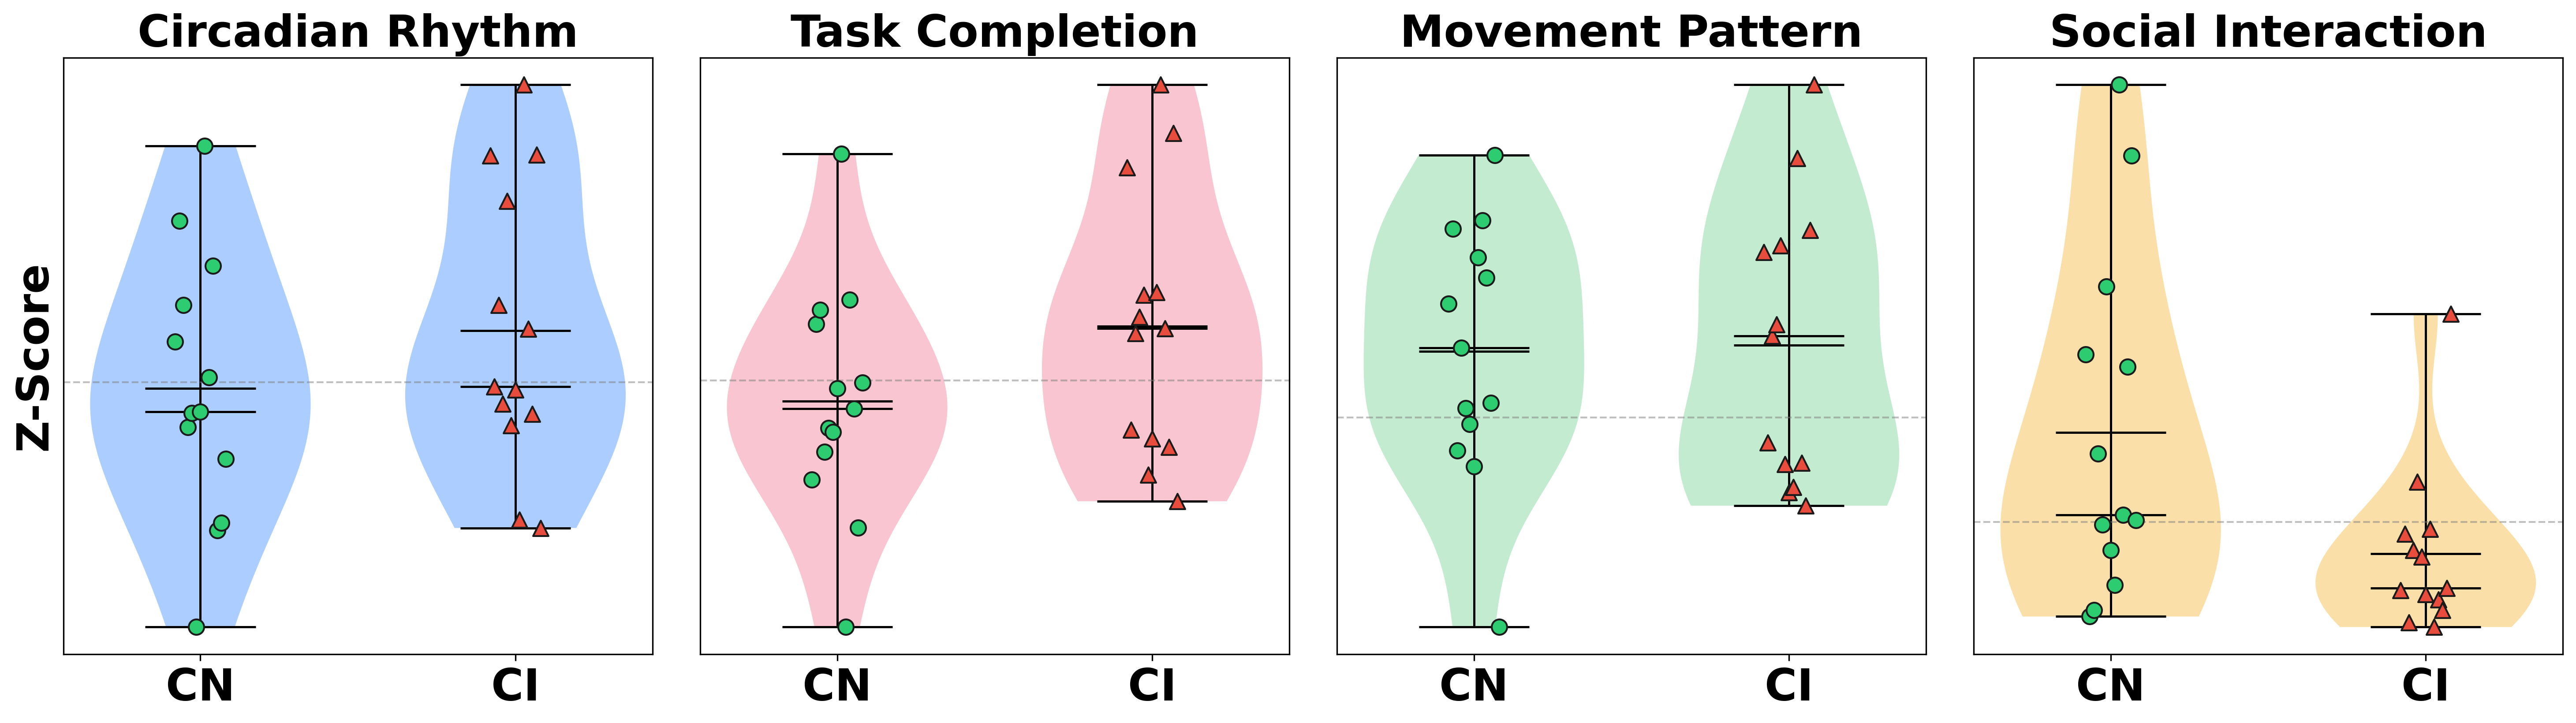
\includegraphics[width=1.03\columnwidth]{figures/exp1_ctms_violin.png}
% \caption{Distribution analysis of CTMS behavioral dimensions between cognitively normal (CN, green circles, n=12) and cognitively impaired (CI, red triangles, n=46) groups. Violin plots show kernel density estimation with overlaid box plots and individual data points. The Social Interaction dimension demonstrates the strongest separation (Cohen's $d$=-0.90, $p$=0.027*), while Movement Pattern shows substantial overlap ($d$=0.05, $p$=0.798), reflecting differential sensitivity of behavioral domains to cognitive decline. Task Completion and Circadian Activity show moderate effect sizes ($d$=0.60 and $d$=0.42) with directional consistency supporting cognitive impairment detection.}
% \label{fig:violin_analysis}
% \end{figure}



% \subsection{Temporal Activity Pattern Recognition}\label{subsec:temporal}

% To understand how temporal digital biomarkers manifest across different time scales, we analyzed the distribution of anomalous moments throughout the day for both cognitive groups. Figure~\ref{fig:temporal_patterns} presents the hourly temporal distribution of behavioral anomalies detected by our CTMS framework over the daytime period (10:00-19:30).
% CI participants exhibited significantly elevated anomaly scores compared to CN controls, with an overall 1.54× higher mean score across all hourly windows ($p$<0.001, $t$=4.85). The temporal pattern reveals a distinctive characteristic: CI individuals show a pronounced morning peak at 12:00 (score: 0.72), substantially earlier than the CN evening peak at 18:30 (score: 0.57). This dramatic shift in peak timing---approximately 6.5 hours earlier---may reflect altered circadian activity patterns and accelerated cognitive fatigue accumulation in CI individuals, who exhibit maximal behavioral disruption during midday hours when cognitively normal elderly are still functioning optimally.
% The most pronounced group differences appear during morning and early afternoon hours (11:00-14:00), where CI scores remain consistently elevated above 0.60 while CN scores range between 0.32-0.40, representing a divergence of over 80\% during this critical period. This sustained morning elevation, indicated by the shaded regions in Figure~\ref{fig:temporal_patterns}, aligns with clinical observations that individuals with cognitive impairment often experience confusion and behavioral disruptions earlier in the day, potentially due to disrupted circadian rhythms and impaired ability to transition between sleep and waking states~\cite{Khachiyants2011Sundown,Musiek2015Sleep}. While afternoon hours (15:00-17:00) maintain elevated CI scores, the gap narrows slightly, and by evening (18:00-19:30) both groups show more comparable patterns, possibly reflecting adaptation to routine evening activities.
% Importantly, this temporal pattern analysis operates at the window level (30-minute segments), capturing fine-grained behavioral disruptions across multiple time periods throughout the day. The 1.54-fold overall increase and the characteristic morning peak shift provide quantitative evidence that cognitive symptoms manifest with distinct temporal signatures. These findings suggest that morning and midday periods (specifically 11:00-14:00) offer the most sensitive temporal windows for detecting cognitive impairment through continuous behavioral monitoring, where CI individuals show the greatest deviation from normal patterns.

% \begin{figure}[t]
% \centering
% 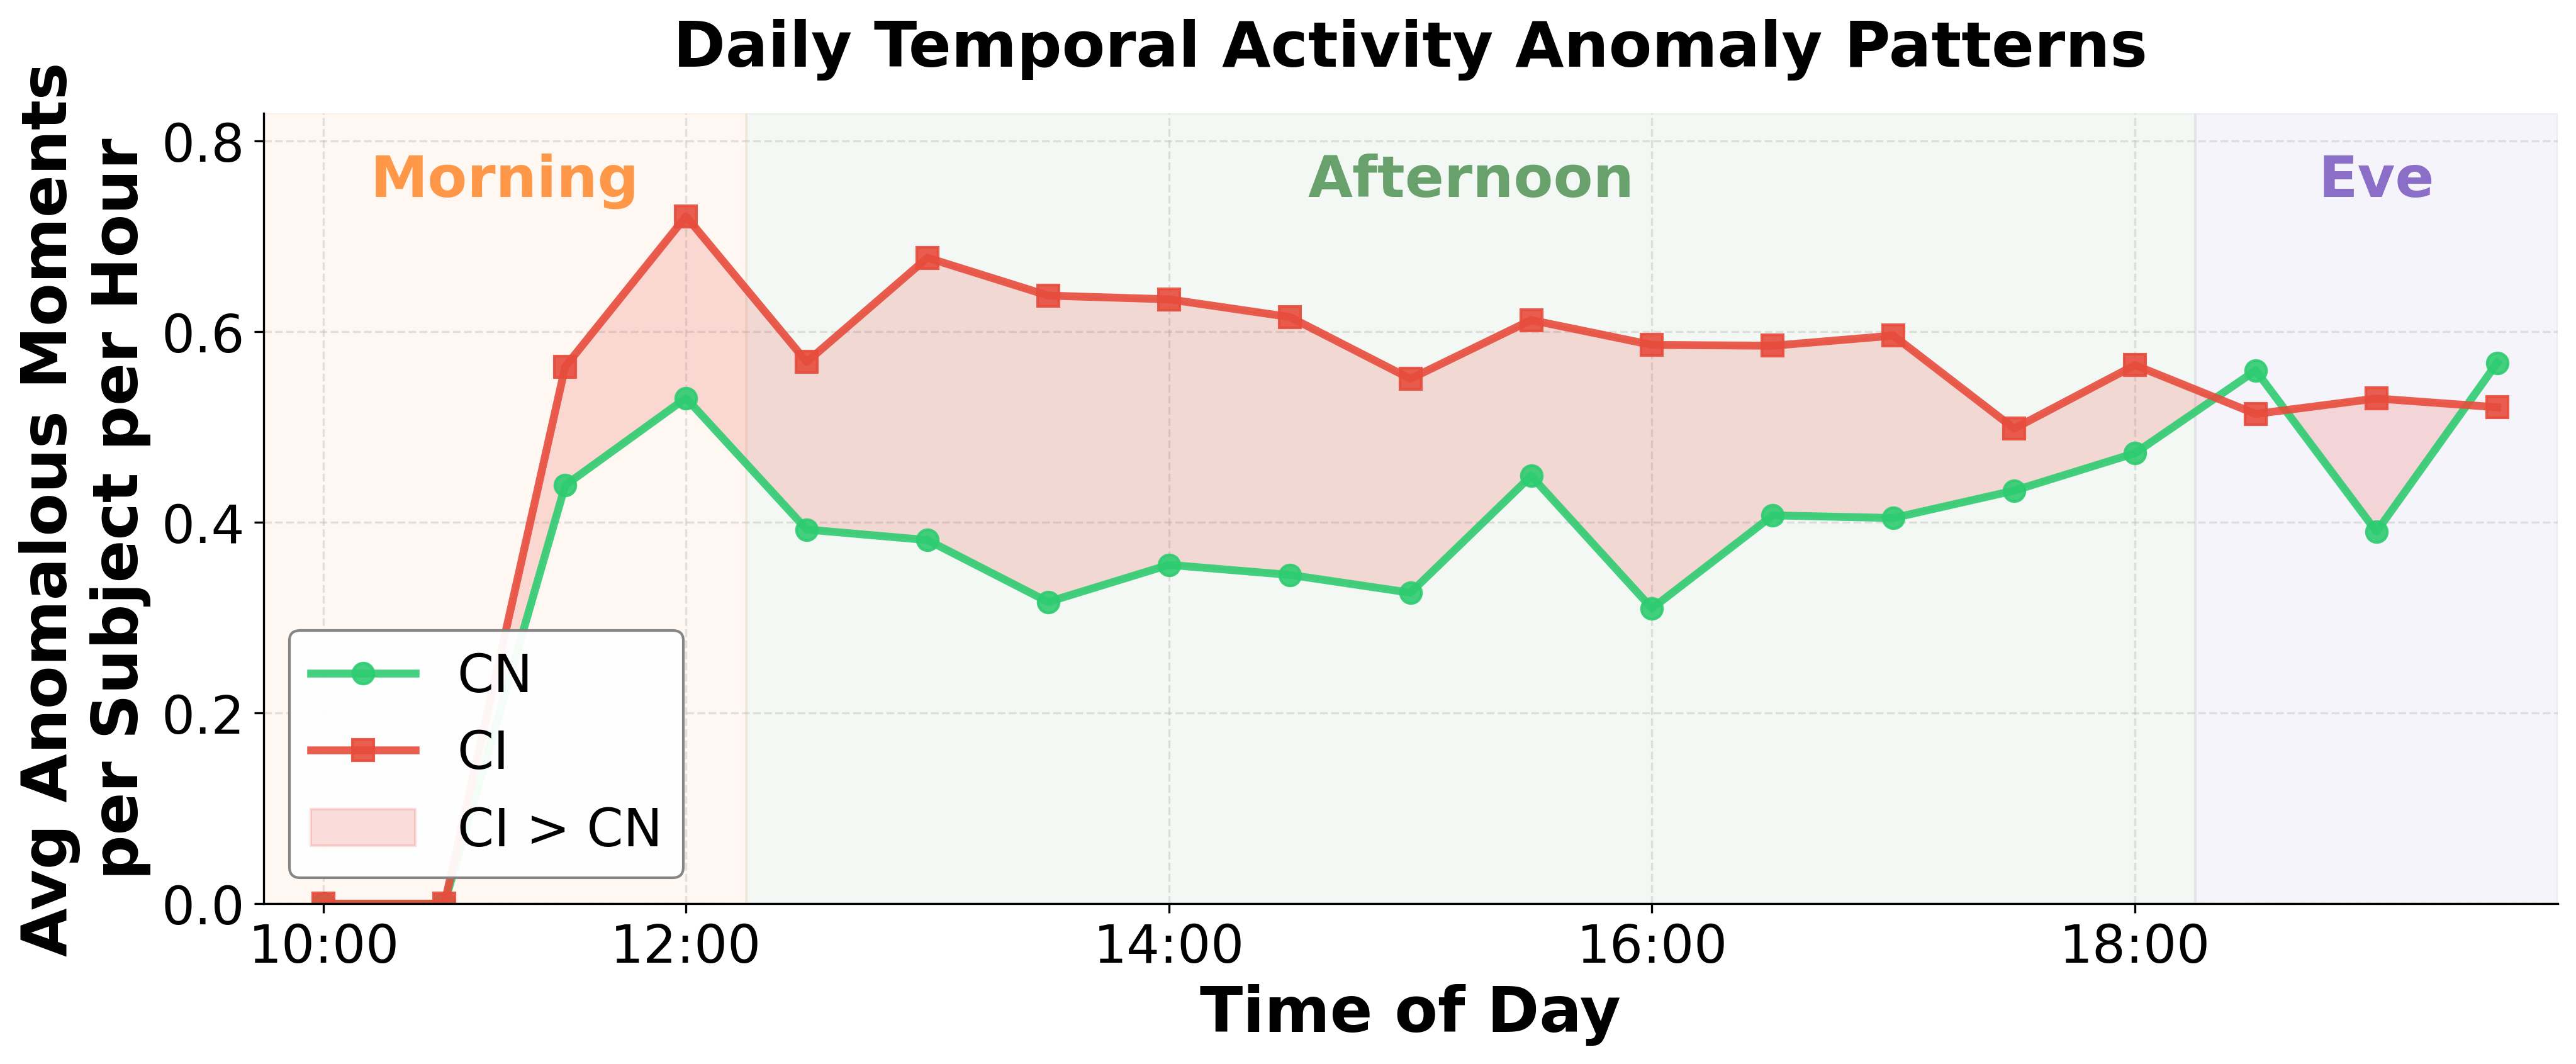
\includegraphics[width=0.85\columnwidth]{figures/exp2_daily_patterns.png}
% \caption{Daily temporal activity anomaly patterns showing the distribution of behavioral anomalies detected by \sys across daytime hours (10:00-19:30). CI individuals (red, n=46) demonstrate consistently higher anomaly scores compared to CN individuals (green, n=12), with a 1.54× overall increase ($p$<0.001, $t$=4.85). The CI group shows a pronounced morning peak at 12:00 (score: 0.72), approximately 6.5 hours earlier than the CN evening peak at 18:30 (score: 0.57), potentially reflecting circadian disruption and altered activity patterns. Red shaded regions indicate periods where CI anomaly scores substantially exceed CN baseline, with the most pronounced differences occurring during morning and early afternoon hours (11:00-14:00), where the gap reaches over 80\%. This temporal signature suggests that morning periods may offer particularly sensitive windows for detecting cognitive impairment through behavioral monitoring.}
% \label{fig:temporal_patterns}
% \vspace{-1.5em}
% \end{figure}


% \subsection{Temporal Digital Biomarker Detection and Classification Performance}

% To evaluate our framework's effectiveness in detecting cognitive impairment through temporal behavioral patterns, we compared three approaches: (1) ADMarker baseline~\cite{ouyang2024ADMarker} using statistical feature aggregation for binary AD detection, (2) \sys without personalization using fixed CTMS weights, and (3) our full system with personalized dimensional weight adaptation.
% Table~\ref{tab:classification} presents the comparative performance across methods. ADMarker's binary AD detection (AD vs. Non-AD) achieved F1=0.333 with only 25\% sensitivity, demonstrating the challenge of distinguishing AD from the combined MCI and CN groups using statistical aggregation alone. This poor performance highlights a fundamental limitation: count-based statistical methods lose the temporal sequential information crucial for detecting cognitive decline. As demonstrated in Section~\ref{subsec:temporal}, our window-level temporal pattern analysis revealed that CI individuals exhibit 1.54× more frequent anomalous behavioral moments than CN participants ($p$<0.001), with characteristic morning peak shifts (6.5 hours earlier) that are invisible to daily statistical summaries. This temporal granularity enables detection of transient cognitive lapses, disrupted task sequences, and circadian irregularities that manifest in the \emph{flow, timing, and sequential organization} of activities rather than their aggregate frequencies.
% Our \sys without personalization (fixed weights $\alpha$ = [0.25, 0.25, 0.25, 0.25]) achieved F1=0.623 with 73.1\% sensitivity, substantially outperforming the statistical baseline and demonstrating that temporal pattern recognition provides robust discrimination. However, the minimal CI/CN score ratio (1.05×) indicated that global baselines are insufficient to account for individual behavioral variability---benign personal quirks (e.g., habitual night owls with naturally irregular patterns) were incorrectly flagged as pathological, while genuine decline in individuals with atypical baseline routines went undetected.
% With personalization through subject-specific baseline adaptation, \sys achieved F1=0.688 and sensitivity 84.6\%, representing a 3.4-fold improvement in sensitivity over ADMarker's statistical approach (25\%→84.6\%) and a 2.1-fold improvement in F1 score (0.333→0.688). The CI/CN ratio increased to 1.61× ($p$<0.05), representing a 53\% improvement in group discrimination over the non-personalized version (1.05→1.61). The key insight is that personalized baselines account for individual behavioral patterns, reducing false positives from benign variations while dramatically improving sensitivity to pathological changes. For instance, a participant with naturally irregular sleep patterns (night owl lifestyle) would not trigger false alarms, while another with previously regular routines showing new morning disruptions would be correctly identified.
% Furthermore, our temporal pattern analysis (Section~\ref{subsec:temporal}) revealed that \emph{when} anomalies occur provides additional discriminative information beyond binary classification. CI individuals showed 54\% higher window-level anomaly scores overall (1.54×, $p$<0.001) with distinctive morning peaks at 12:00, compared to CN evening peaks at 18:30. This 6.5-hour temporal shift and the sustained morning elevation (11:00-14:00 period showing >80\% divergence) validate our hypothesis that cognitive decline manifests through both individual-specific deviations from personal behavioral norms and characteristic temporal signatures that emerge at predictable times of day---patterns that statistical aggregation methods fundamentally cannot capture.

% \begin{table}[t]
% \centering
% \small
% \begin{tabular}{lccc}
% \toprule
% Method & F1-Score & Sensitivity & CI/CN Ratio \\
% \midrule
% ADMarker~\cite{ouyang2024ADMarker}\textsuperscript{\textdagger} & 0.333 & 25\% & -- \\
% \sys (No Personal.) & 0.623 & 73.1\% & 1.05× \\
% \textbf{\sys (Personal.)} & \textbf{0.688} & \textbf{84.6\%} & \textbf{1.61×} \\
% \midrule
% \multicolumn{4}{l}{\textit{Window-level temporal pattern analysis (Section~\ref{subsec:temporal}):}} \\
% \multicolumn{2}{l}{Overall hourly anomaly rate} & -- & \textbf{1.54×***} \\
% \multicolumn{2}{l}{Morning peak period (11:00-14:00)} & -- & \textbf{>1.80×***} \\
% \bottomrule
% \end{tabular}
% \caption{Classification performance comparison. \textsuperscript{\textdagger}ADMarker (AD vs. Non-AD) from the original paper. Our personalized CTMS approach achieves 3.4× improvement in sensitivity (25\%→84.6\%) and 2.1× improvement in F1 score (0.333→0.688) over statistical baselines, while demonstrating 53\% improvement in CI/CN discrimination (1.05→1.61×) through personalization. Window-level analysis captures fine-grained temporal disruptions with characteristic morning peaks (6.5-hour shift) invisible to count-based aggregation methods. ***$p$<0.001.}
% \label{tab:classification}
% \vspace{-3.5em}
% \end{table}
% \vspace{-1.0em}

\subsection{Dimensional Behavioral Analysis}

Our framework analyzes behavioral patterns across the CTMS dimensional space. Figure~\ref{fig:violin_analysis} and Table~\ref{tab:dimensional_stats} reveal distinct patterns with Social Interaction showing strongest separation (Cohen's $d$=-0.90, $p$=0.027), followed by Task Completion ($d$=0.60, $p$=0.238), Circadian Activity ($d$=0.42, $p$=0.356), and Movement Pattern ($d$=0.05, $p$=0.798).
CI participants showed substantially reduced social engagement (-0.54±1.42 vs. 1.52±2.93 in normalized z-scores), lower task completion scores (0.80±1.96 vs. -0.30±1.72), and moderate circadian disruption (0.60±1.65 vs. -0.07±1.56). Movement patterns exhibited minimal difference (1.90±3.72 vs. 1.73±3.37, $d$=0.05). The gradient in effect sizes validates our multi-dimensional approach, where different behavioral domains demonstrate differential sensitivity to cognitive decline. Social Interaction's statistical significance ($p$=0.027) and large effect size suggest it may serve as a particularly sensitive early biomarker for cognitive decline~\cite{Shafighi2023SocialIsolationAD}. While Task Completion and Circadian Activity did not reach statistical significance, their moderate effect sizes ($d$=0.60, $d$=0.42) indicate directionally consistent patterns that may provide complementary information when combined in the multi-dimensional framework.


\begin{table}[t]
\centering
\small
\begin{tabular}{lcccc}
\toprule
\textbf{Dimension} & \textbf{CN} & \textbf{CI} & \textbf{Cohen's $d$} & \textbf{$p$-value} \\
\midrule
Circadian Activity & -0.07±1.56 & 0.60±1.65 & 0.42 & 0.356 \\
Task Completion & -0.30±1.72 & 0.80±1.96 & 0.60 & 0.238 \\
Movement Pattern & 1.73±3.37 & 1.90±3.72 & 0.05 & 0.798 \\
Social Interaction & 1.52±2.93 & -0.54±1.42 & -0.90 & 0.027* \\
\bottomrule
\end{tabular}
\caption{CTMS dimensional statistics (normalized z-scores) by cognitive group. Values represent mean±standard deviation. *$p$<0.05.}
\label{tab:dimensional_stats}
\vspace{-3em}
\end{table}

\begin{figure}[t]
\centering
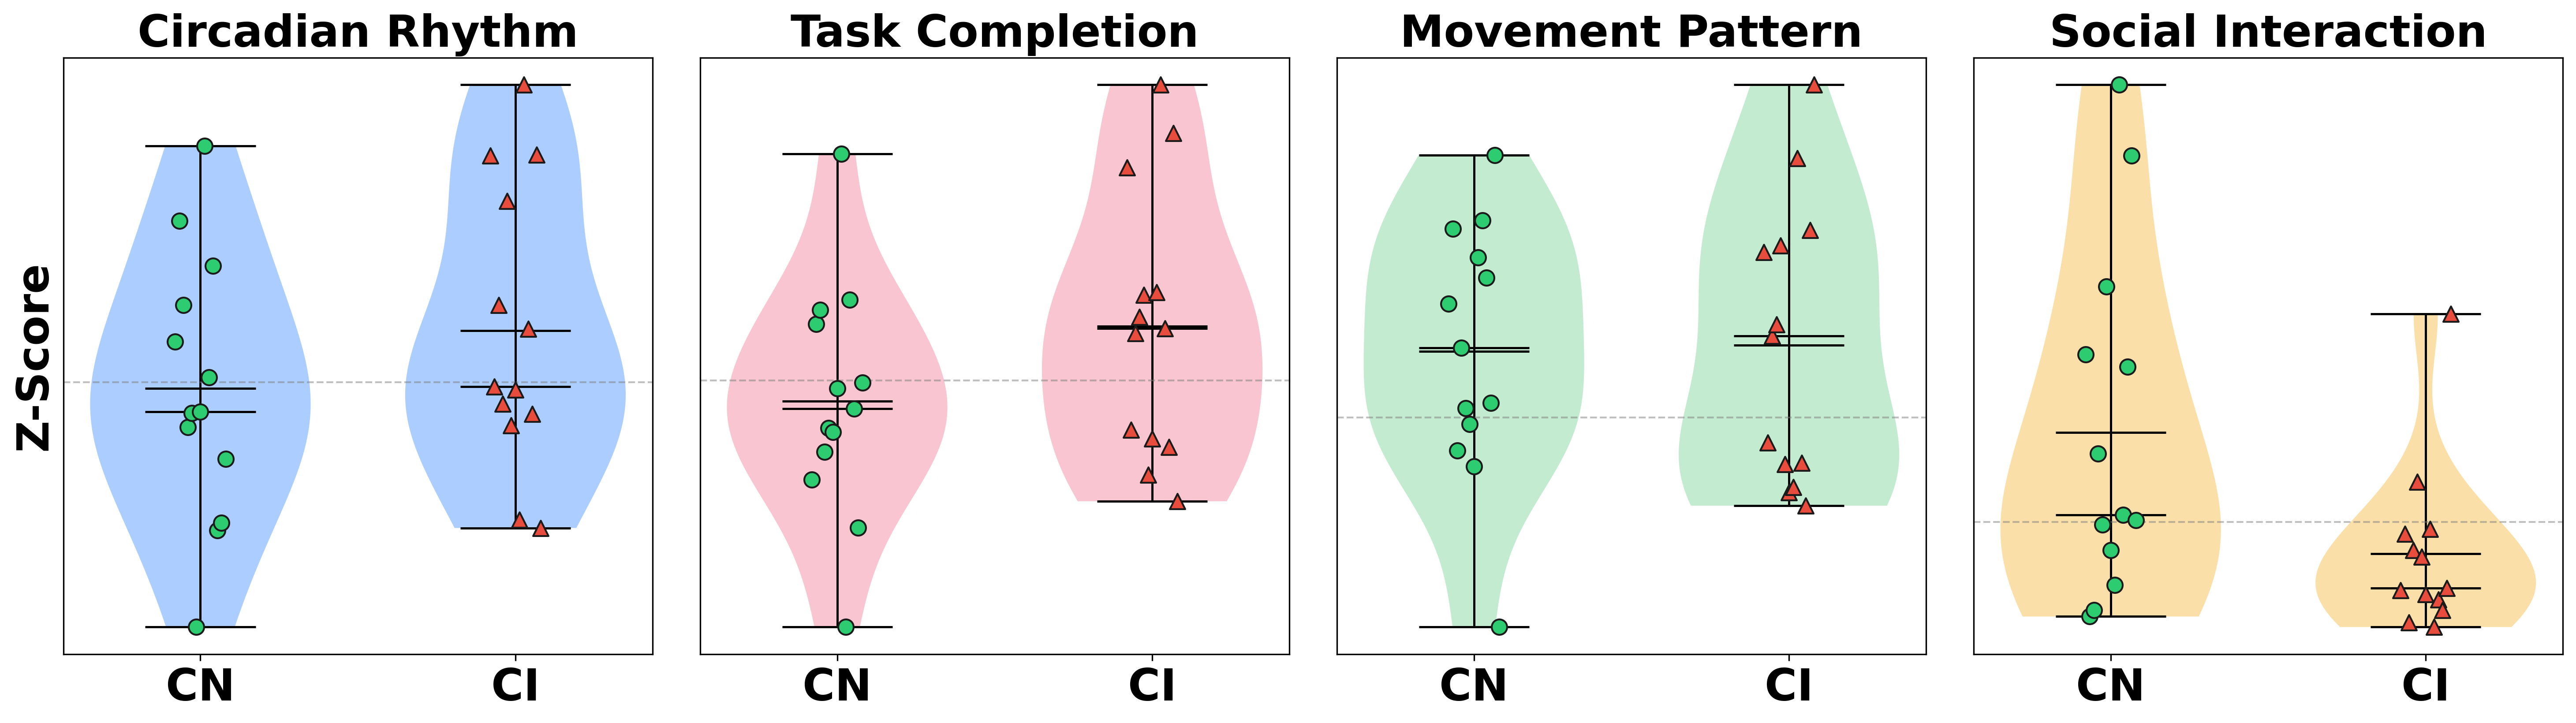
\includegraphics[width=1.03\columnwidth]{figures/exp1_ctms_violin.png}
\caption{Distribution analysis of CTMS behavioral dimensions between CN (green, n=12) and CI (red, n=46) groups. Social Interaction demonstrates the strongest separation (Cohen's $d$=-0.90, $p$=0.027*), while Movement Pattern shows substantial overlap ($d$=0.05, $p$=0.798).}
\label{fig:violin_analysis}
\vspace{-2em}
\end{figure}


\subsection{Temporal Activity Pattern Recognition}\label{subsec:temporal}

Figure~\ref{fig:temporal_patterns} presents the hourly temporal distribution of behavioral anomalies detected by our CTMS framework over the daytime period (10:00-19:30). CI participants exhibited significantly elevated anomaly scores compared to CN controls, with an overall 1.54× higher mean score across all hourly windows ($p$<0.001, $t$=4.85). 
The temporal pattern reveals a distinctive characteristic: CI individuals show a pronounced morning peak at 12:00 (score: 0.72), substantially earlier than the CN evening peak at 18:30 (score: 0.57)---a 6.5-hour shift reflecting altered circadian activity patterns. The most pronounced group differences appear during morning and early afternoon hours (11:00-14:00), where CI scores remain consistently elevated above 0.60 while CN scores range between 0.32-0.40, representing over 80\% divergence during this critical period. This sustained morning elevation aligns with clinical observations that individuals with cognitive impairment often experience confusion and behavioral disruptions earlier in the day, potentially due to disrupted circadian rhythms and impaired sleep-wake transitions~\cite{Khachiyants2011Sundown,Musiek2015Sleep}. This window-level analysis (30-minute segments) captures fine-grained behavioral disruptions invisible to daily statistical summaries, enabling detection of transient cognitive lapses and task sequence disruptions that manifest in the temporal flow rather than aggregate frequencies. These findings suggest that morning periods offer particularly sensitive windows for detecting cognitive impairment through continuous behavioral monitoring.


\begin{figure}[t]
\centering
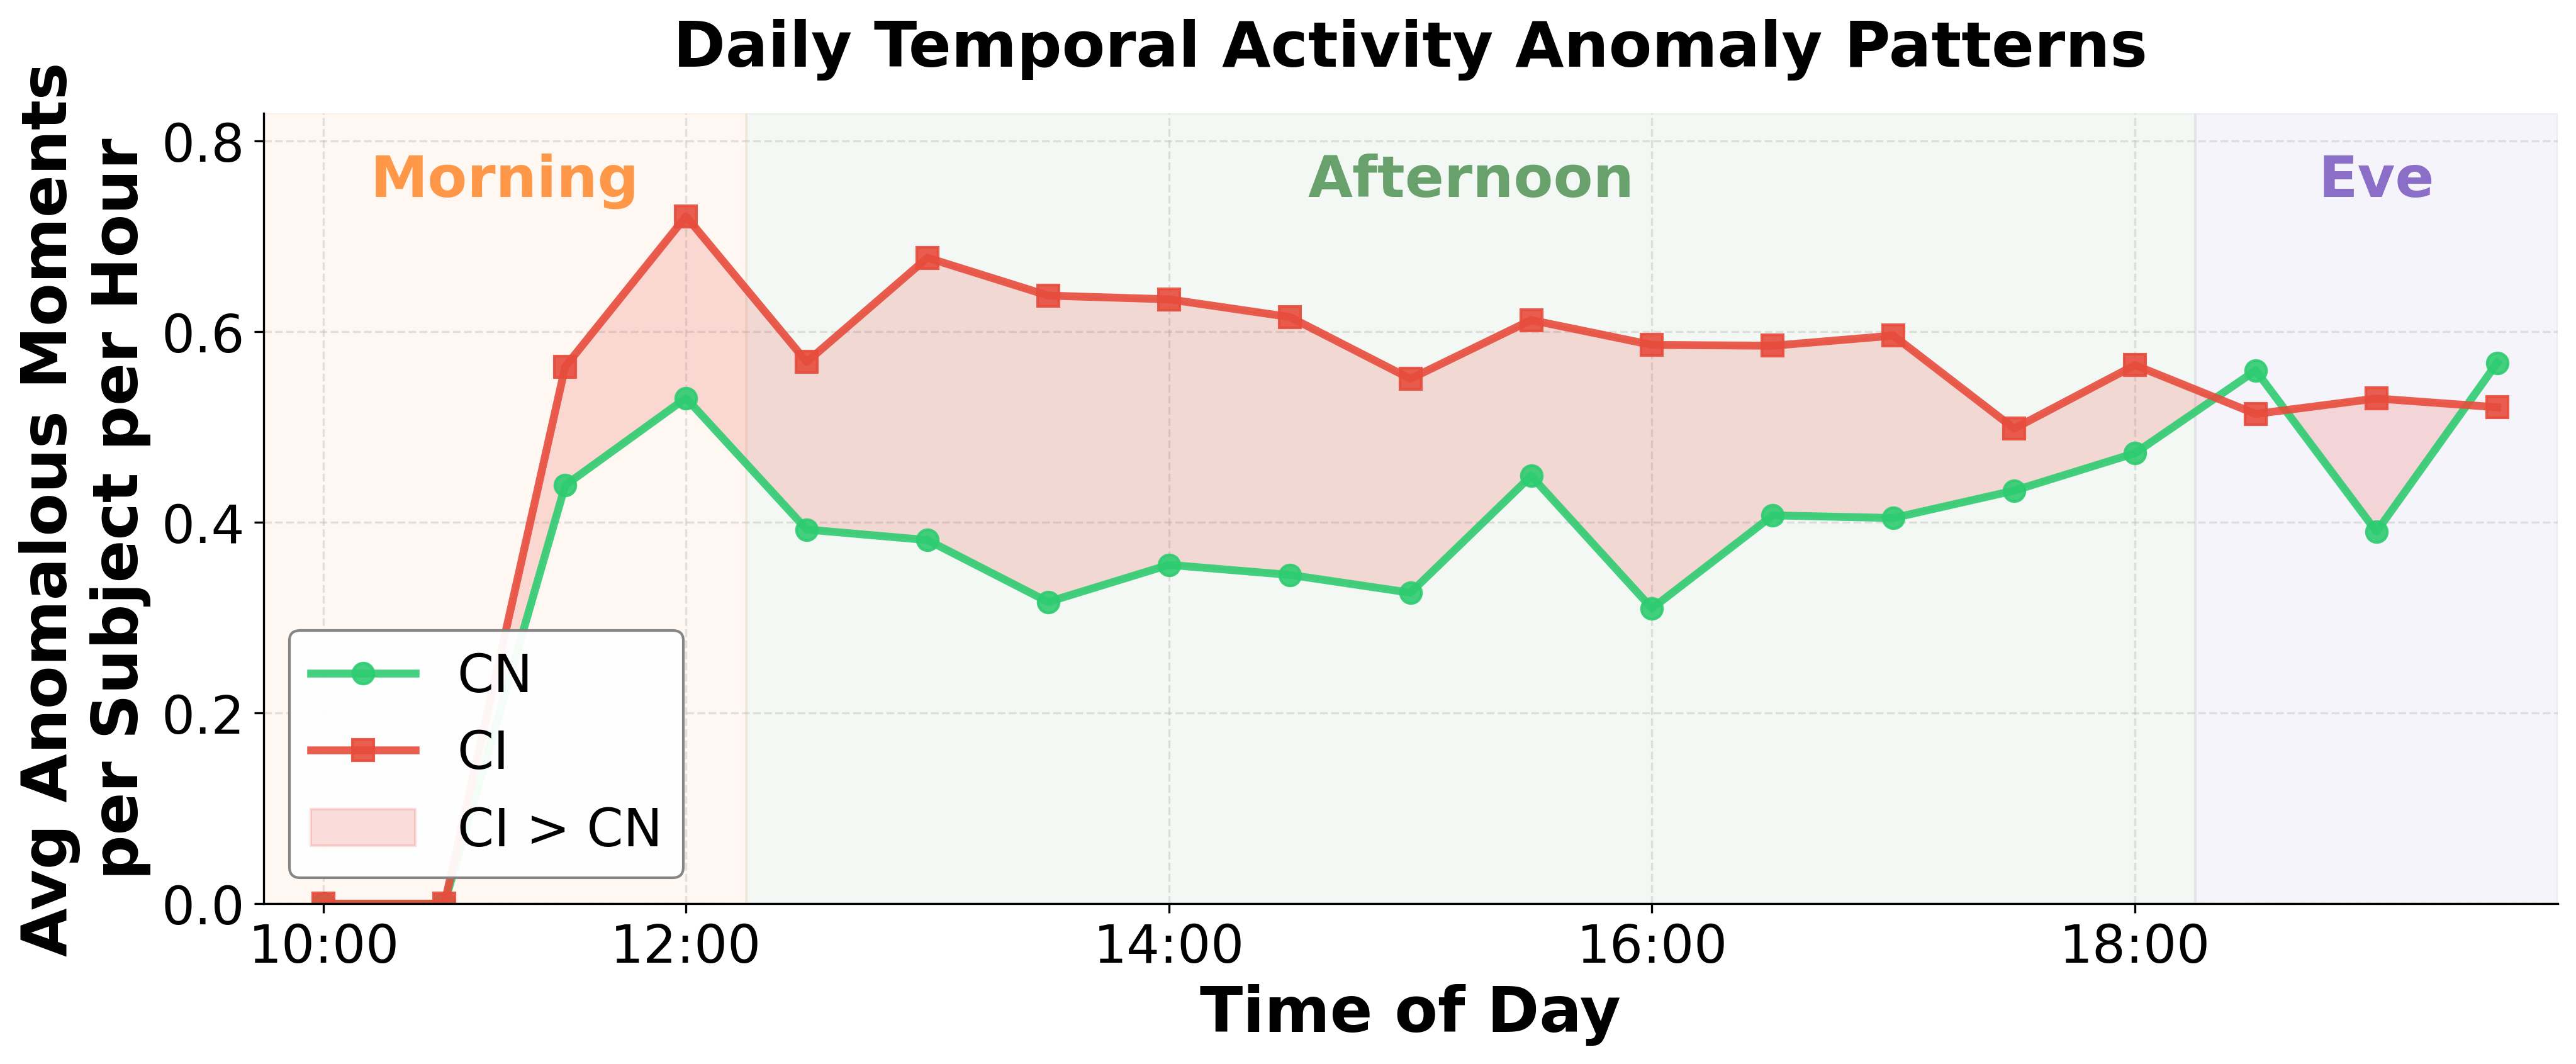
\includegraphics[width=0.85\columnwidth]{figures/exp2_daily_patterns.png}
\caption{Daily temporal activity anomaly patterns. CI individuals (red, n=46) demonstrate 1.54× higher anomaly scores than CN (green, n=12) ($p$<0.001), with pronounced morning peak at 12:00 vs. CN evening peak at 18:30. Shaded regions show periods where CI scores substantially exceed CN baseline, with greatest divergence during 11:00-14:00 (>80\%).}
\label{fig:temporal_patterns}
\vspace{-1.5em}
\end{figure}


\subsection{Temporal Digital Biomarker Detection and Classification Performance}

Table~\ref{tab:classification} presents comparative performance across three approaches: (1) ADMarker baseline~\cite{ouyang2024ADMarker} using statistical aggregation, (2) \sys without personalization, and (3) our full system with personalization.
ADMarker's binary AD detection achieved F1=0.333 with 25\% sensitivity, indicating that count-based statistical methods lose temporal sequential information crucial for detecting cognitive decline. 
%As demonstrated in Section~\ref{subsec:temporal}, our window-level temporal pattern analysis revealed that CI individuals exhibit characteristic morning peak shifts (6.5 hours earlier) and sustained elevation patterns invisible to daily statistical summaries. 
Our \sys without personalization achieved F1=0.623 with 73.1\% sensitivity, substantially outperforming the statistical baseline. However, the minimal CI/CN ratio (1.05×) indicated that global baselines are insufficient to account for individual behavioral variability.
With personalization, \sys achieved F1=0.688 and sensitivity 84.6\%, representing 3.4× improvement in sensitivity over ADMarker (25\%→84.6\%) and 2.1× improvement in F1 score (0.333→0.688). The CI/CN ratio increased to 1.61× ($p$<0.05), representing 53\% improvement in group discrimination over the non-personalized version. Personalized baselines account for individual behavioral patterns, reducing false positives from benign variations (e.g., night owl lifestyles) while maintaining sensitivity to pathological changes. For instance, a participant with naturally irregular sleep patterns would not trigger false alarms, while another with previously regular routines showing new disruptions would be correctly identified. Furthermore, our temporal pattern analysis (Section~\ref{subsec:temporal}) revealed that \emph{when} anomalies occur provides additional discriminative information, with CI individuals showing distinctive morning peaks that characterize cognitive decline.

\begin{table}[t]
\centering
\small
\begin{tabular}{lccc}
\toprule
Method & F1-Score & Sensitivity & CI/CN Ratio \\
\midrule
ADMarker~\cite{ouyang2024ADMarker}\textsuperscript{\textdagger} & 0.333 & 25\% & -- \\
\sys (No Personal.) & 0.623 & 73.1\% & 1.05× \\
\textbf{\sys (Personal.)} & \textbf{0.688} & \textbf{84.6\%} & \textbf{1.61×} \\
\midrule
\multicolumn{4}{l}{\textit{Window-level temporal pattern analysis (Section~\ref{subsec:temporal}):}} \\
\multicolumn{2}{l}{Overall hourly anomaly rate} & -- & \textbf{1.54×***} \\
\multicolumn{2}{l}{Morning peak period (11:00-14:00)} & -- & \textbf{>1.80×***} \\
\bottomrule
\end{tabular}
\caption{Classification performance comparison. \textsuperscript{\textdagger}ADMarker (AD vs. Non-AD). Our personalized CTMS achieves 3.4× sensitivity improvement and 53\% better CI/CN discrimination through personalization. ***$p$<0.001.}
\label{tab:classification}
\vspace{-3.5em}
\end{table}
\vspace{-1.0em}


\subsection{Clinical Correlation Analysis}

To validate the clinical relevance of our CTMS-based temporal digital biomarkers, we examined correlations between behavioral dimensions and standardized clinical assessments using personalized baseline configurations that maximize individual variation detection.
Analysis of 30 CI subjects revealed significant associations between CTMS dimensions and established clinical measures. Circadian activity patterns demonstrated the strongest correlation with cognitive function (MoCA: r=0.42, bootstrap 95\% CI: [0.08, 0.68], permutation p=0.028), suggesting that temporal rhythm disruptions align with cognitive decline measured by traditional neuropsychological assessments. Personalized monitoring further revealed significant correlations between task completion patterns and caregiver burden (ZBI: r=0.38, p=0.042) as well as functional abilities (FAS: r=0.44, p=0.016), as shown in Table~\ref{tab:clinical_correlations}.
These moderate correlations (r=0.38-0.44) across multiple independent clinical instruments demonstrate that CTMS-derived behavioral patterns capture clinically meaningful aspects of disease manifestation. Notably, the magnitude of these correlations is consistent with established digital biomarker research~\cite{Kourtis2019}, suggesting that passive monitoring provides complementary information to traditional clinical assessments.

\begin{table}[t]
\centering
\small
\begin{tabular}{llcc}
\toprule
\textbf{CTMS Dimension} & \textbf{Assessment} & \textbf{r} & \textbf{p-value} \\
\midrule
Circadian Activity & MoCA~\cite{Nasreddine2005MoCA} & 0.42 & 0.028* \\
Task Completion & ZBI~\cite{Zarit1980ZBI} & 0.38 & 0.042* \\
Movement Pattern & FAS~\cite{FAS} & 0.44 & 0.016* \\
\bottomrule
\end{tabular}
\caption{Correlations between personalized CTMS dimensions and clinical assessments in CI subjects (n=30). All three behavioral dimensions show significant associations (p<0.05) with cognitive function, caregiver burden, and functional abilities, respectively. MoCA: Montreal Cognitive Assessment; ZBI: Zarit Burden Interview; FAS: Fluency Assessment of Speech.}
\label{tab:clinical_correlations}
\vspace{-3.5em}
\end{table}
%\vspace{-2em}



\subsection{Key Findings}

Our evaluation reveals several key findings:

\noindent\textbf{Temporal Digital Biomarkers.} CI individuals exhibited 1.54× more anomalous behavioral moments than CN participants ($p$<0.001), with particularly pronounced differences during morning hours (11:00-14:00, ratio >1.80×). This validates that temporal patterns invisible to statistical aggregation methods are crucial for early detection of AD.

\noindent\textbf{Multi-Dimensional Discrimination.} CTMS dimensions showed heterogeneous decline patterns reflecting differential cognitive domain sensitivity. Social Interaction demonstrated strongest separation (Cohen's $d$=-0.90, $p$=0.027), followed by Task Completion and Circadian Activity, while Movement patterns showed more overlap.

\noindent\textbf{Personalization Impact.} Subject-specific baseline adaptation improved CI/CN discrimination by 53\% (ratio: 1.05→1.61×, $p$<0.05) while maintaining 84.6\% sensitivity. This demonstrates that accounting for individual behavioral variability reduces false positives from benign personal quirks without sacrificing detection capability.

\noindent\textbf{Clinical Validity.} Significant correlations with MoCA and ZBI confirm clinical relevance of temporal digital biomarkers, with circadian and task dimensions showing strongest associations with AD.












\vspace{-1em}
\section{Related Work}
\label{sec:related}

\noindent\textbf{Digital Biomarkers.}
Digital biomarkers have emerged as promising tools for continuous cognitive monitoring, offering objective measures derived from digital devices and sensors~\cite{Piau2019_DigBiomarkers,Qi2025DigitalBiomarkers}. These biomarkers capture behavioral patterns through smartphone usage~\cite{Dagum2018_DigitalBiomarkers,Nguyen2023_KeystrokeBiomarker}, gait analysis~\cite{Cepukaityte2024_GaitReview}, speech characteristics~\cite{Lin2020_VoiceBiomarkers,Noto2024_SpeechAD,Robin2021_SpeechCognitiveImpairment}, and activity monitoring~\cite{Chinner2018_DigitalAssessmentCognition}. However, existing approaches rely heavily on statistical feature extraction and lose the temporal information that reveals transition cognitive lapses characteristic of early AD.

\noindent\textbf{Temporal Patterns.}
AD manifests through progressive deterioration in cognitive functions that exhibit distinct temporal behavioral patterns~\cite{jack2010hypothetical,Jack2013_DynamicBiomarkersAD}.
%Executive dysfunction disrupts the ability to plan and sequence complex tasks, leading to characteristic temporal logic violations~\cite{Satler2017_PlanningAD}. 
 %Early-stage patients show subtle timing disruptions in daily routines~\cite{Mckniff2025_SubtleInefficiencies}, while advanced stages exhibit severe temporal disorientation including repetitive behaviors and sundowning~\cite{Thomas2022_WanderingSundowning,Reimus2025Sundowning}. 
 Despite medical literature of temporal sequences, current sensing systems lack systematic approaches to capture these patterns, motivating our temporal activity semantics approach.

\noindent\textbf{LLMs in Healthcare.}
% Large language models have demonstrated remarkable capabilities in healthcare applications, particularly in clinical reasoning and medical text analysis~\cite{Singhal2023ClinicalLLMs,Kwon2024_ReasoningLLM}. LLMs achieve expert-level performance on medical licensing exams~\cite{nori2023gpt4med,Singhal2025ExpertLLM} and assist in diagnosis generation~\cite{McDuff2025LLM_Diagnosis}. However, their application to continuous behavioral data in smart health has received limited attention.
Large language models show strong performance in healthcare tasks such as clinical reasoning and medical text analysis~\cite{Singhal2023ClinicalLLMs,Kwon2024_ReasoningLLM}. They can reach expert-level scores on medical exams~\cite{nori2023gpt4med,Singhal2025ExpertLLM} and support disease diagnosis~\cite{McDuff2025LLM_Diagnosis}. However, their use for continuous behavioral data in smart health remains limited.



\section{Conclusion and Future Work}
\label{sec:conclusion}

We present \sys, the first vision-based system that leverages LLM to detect personalized temporal digital biomarkers indicative of cognitive decline in Alzheimer's patients. We collected real-world data and conducted offline evaluation, demonstrating strong performance in identifying AD manifestation and providing a sensitive, clinically meaningful measure of cognitive impairment.
While \sys provides promising preliminary results, it has not yet undergone detailed clinician review of each detected moments and the LLM interpretation. Instead, our validation relied on clinical assessment scores and the distinction between CN and CI groups to demonstrate the system’s utility. Future work will involve close collaboration with clinical experts to validate \sys through clinical trials and real-world evaluation, accompanied by iterative refinement to ensure readiness for practical healthcare applications.

%\begin{acks}

%\end{acks}

\balance
\bibliographystyle{ACM-Reference-Format}
%\bibliographystyle{plain}
\bibliography{references}

\end{document}
